% =====================================================================
%  Chapitre 1 -- partie b : biais-variance, decoupage, fuite, baseline, TP
% =====================================================================

\begin{frame}{D'où vient l'erreur : biais et variance}
\begin{center}
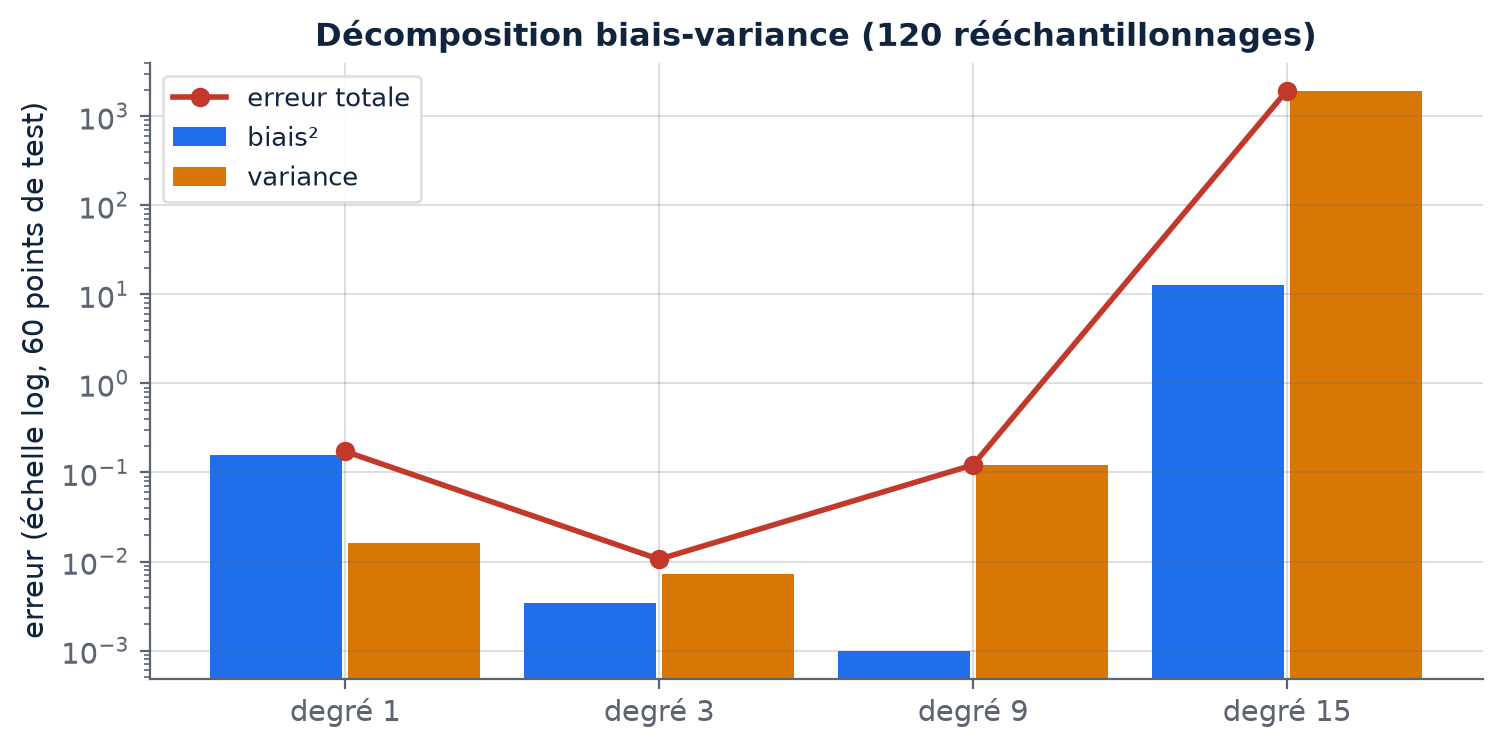
\includegraphics[width=0.84\textwidth]{g04_biais_variance.png}
\end{center}
\vspace{1mm}
\begin{columns}[t]
\begin{column}{0.48\textwidth}
\footnotesize
\textbf{Deux expériences distinctes} (autres tirages que la slide précédente) :
deg.~1 $\rightarrow$ erreur $0{,}173$ dont biais $0{,}156$ ;
deg.~3 $\rightarrow$ $0{,}011$ ;
deg.~9 $\rightarrow$ $0{,}122$ dont variance $0{,}121$.
\end{column}
\begin{column}{0.48\textwidth}
\footnotesize
Au degré 15, la variance atteint \textbf{1\,936} : le modèle change
entièrement d'un échantillon à l'autre. C'est la définition même de
l'instabilité.
\end{column}
\end{columns}
\end{frame}

\begin{frame}{Le dilemme, énoncé proprement}
\begin{center}
\[
  \underbrace{\mathbb{E}\big[(y-\hat f(x))^2\big]}_{\text{erreur attendue}}
  \;=\;
  \underbrace{\text{biais}^2}_{\text{modèle trop simple}}
  \;+\;
  \underbrace{\text{variance}}_{\text{modèle trop souple}}
  \;+\;
  \underbrace{\sigma^2}_{\text{bruit irréductible}}
\]
\end{center}
\begin{columns}[t]
\begin{column}{0.48\textwidth}
\begin{itemize}
  \item Modèle simple : biais fort, variance faible.
  \item Modèle souple : biais faible, variance forte.
\end{itemize}
\end{column}
\begin{column}{0.48\textwidth}
\begin{kbox}[Ce qu'on ne peut pas éviter]
Le terme $\sigma^2$ est le bruit des données. Aucun modèle ne le réduit :
un score parfait sur des données bruitées est un signe de fuite.
\end{kbox}
\end{column}
\end{columns}
\end{frame}

\begin{frame}{Découper les données}
\begin{center}
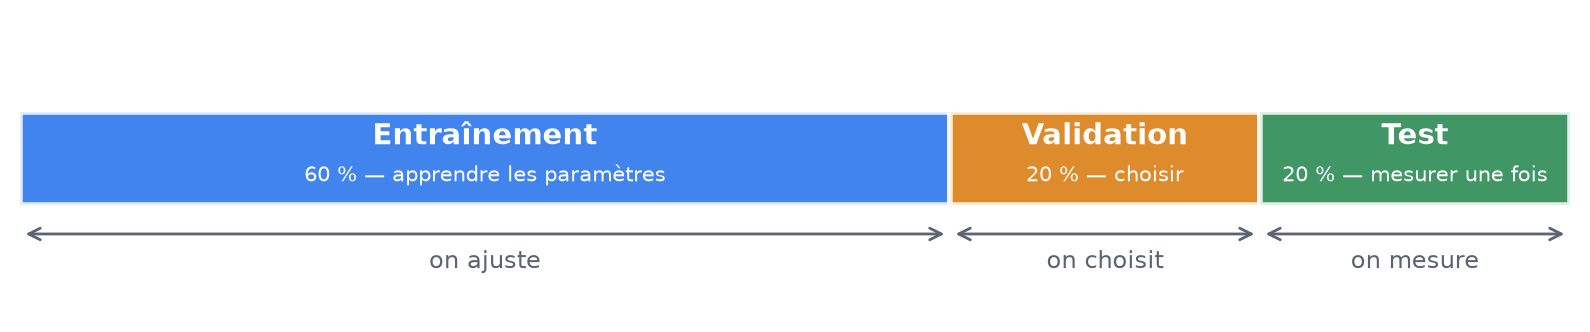
\includegraphics[width=0.95\textwidth]{g05_split.png}
\end{center}
\vspace{1mm}
\begin{columns}[t]
\begin{column}{0.48\textwidth}
\begin{ebox}[Entraînement]
Ajuste les paramètres.
\end{ebox}
\end{column}
\begin{column}{0.48\textwidth}
\begin{ebox}[Validation]
Choisit les hyperparamètres, compare les modèles.
\end{ebox}
\end{column}
\end{columns}
\vspace{1mm}
\begin{wbox}[Le jeu de test ne se touche qu'une fois]
Chaque consultation du test pour choisir un modèle le transforme en jeu de
validation. À la fin, votre score n'est plus une estimation honnête.
\end{wbox}
\end{frame}

\begin{frame}{Validation croisée : quand les données sont rares}
\begin{center}
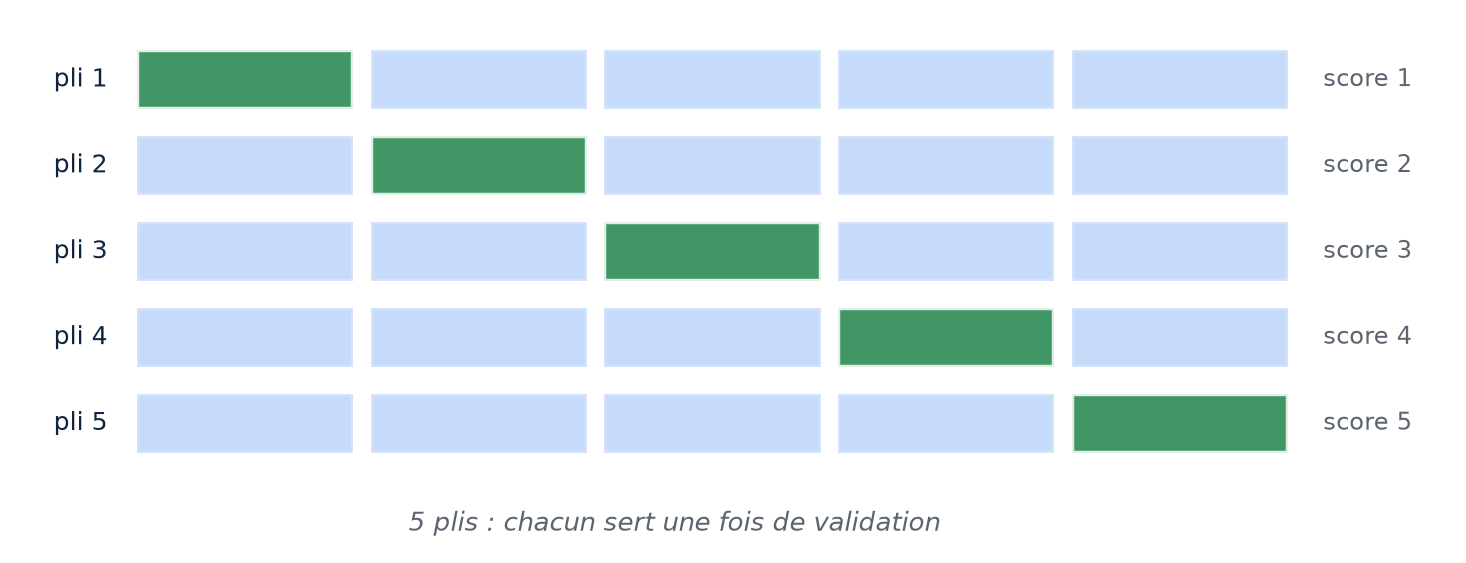
\includegraphics[width=0.9\textwidth]{g06_kfold.png}
\end{center}
\vspace{1mm}
\begin{columns}[t]
\begin{column}{0.52\textwidth}
\begin{itemize}
  \item On découpe en $K$ plis ; chacun sert une fois de validation.
  \item On rapporte la \textbf{moyenne} et l'\textbf{écart-type} des $K$ scores.
  \item $K=5$ ou $10$ : compromis coût / stabilité.
\end{itemize}
\end{column}
\begin{column}{0.44\textwidth}
\begin{wbox}[Le piège du score unique]
Un score unique cache l'instabilité. « $0{,}82 \pm 0{,}06$ » est une
information ; « $0{,}82$ » n'en est pas une.
\end{wbox}
\end{column}
\end{columns}
\end{frame}

\begin{frame}{Une fuite, c'est quoi exactement ?}
\begin{solbox}[Définition]
Il y a \textbf{fuite} quand le modèle dispose, au moment de l'entraînement,
d'une information qu'il \textbf{n'aura pas} au moment de décider.
\end{solbox}
\vspace{1mm}
\begin{columns}[t]
\begin{column}{0.48\textwidth}
\begin{wbox}[Fuite « métier »]
Une variable postérieure à la décision. Exemple : prédire en octobre si un
étudiant réussira, en gardant la colonne « a été convoqué en tutorat en juin ».
Le modèle lit la conséquence, pas la cause.
\end{wbox}
\end{column}
\begin{column}{0.48\textwidth}
\begin{wbox}[Fuite « protocole »]
Le jeu de test influence l'entraînement : moyennes calculées sur tout le
tableau, variables choisies avant le découpage, quasi-doublons répartis des
deux côtés.
\end{wbox}
\end{column}
\end{columns}
\vspace{1mm}
\begin{kbox}[Pourquoi c'est grave]
Le score monte, la décision reste fausse. Une fuite ne se voit pas dans le
notebook : elle se voit dans le \textbf{monde réel}, quand le modèle se trompe
alors que tout semblait parfait.
\end{kbox}
\end{frame}

\begin{frame}{La fuite de données : une expérience}
\begin{columns}[t]
\begin{column}{0.44\textwidth}
\centering
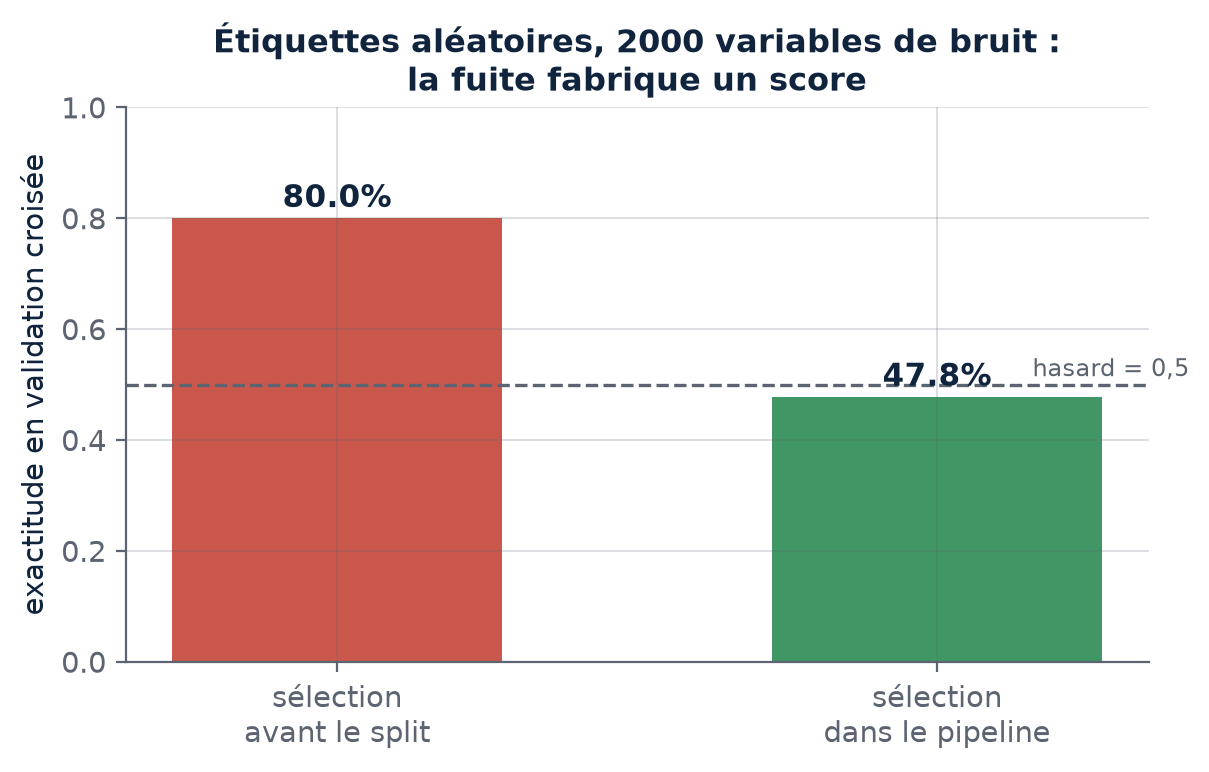
\includegraphics[width=\textwidth]{g07_fuite.png}
\end{column}
\begin{column}{0.52\textwidth}
\begin{wbox}[Le protocole]
$n=90$ patients, $p=2\,000$ variables \textbf{de pur bruit}, étiquettes
tirées au hasard : il n'y a \textbf{rien} à apprendre.
\end{wbox}
\begin{itemize}
  \item Sélection des 12 « meilleures » variables sur \textbf{toutes} les
  données, puis validation croisée : \textbf{80,0 \%}.
  \item Même sélection placée \textbf{dans le pipeline} : \textbf{47,8 \%}.
\end{itemize}
\begin{solbox}[Le mécanisme, en une phrase]
Parmi $2\,000$ colonnes de bruit, certaines sont corrélées à $y$ \textbf{par
hasard} ; les sélectionner sur tout le jeu revient à retenir celles qui
contiennent déjà la réponse. L'écart de \textbf{32 points} ne vient pas du
modèle mais du protocole.
\end{solbox}
\end{column}
\end{columns}
\end{frame}

\begin{frame}{Quatre fuites qui reviennent toujours}
\begin{center}
\small
\footnotesize
\begin{tabular}{@{}p{0.25\textwidth}p{0.22\textwidth}p{0.37\textwidth}@{}}
\toprule
\textbf{Fuite} & \textbf{Famille} & \textbf{Exemple} \\
\midrule
Prétraitement avant le split & protocole & standardiser sur tout le jeu \\
Sélection globale & protocole & garder les colonnes corrélées à $y$ \\
Doublons, scènes identiques & protocole & tuiles d'une même photo, même
patient sur deux semestres \\
Cible déguisée & métier & « a été convoqué en tutorat » \\
Variable postérieure & métier & le montant de la facture pour prédire un
impayé \\
\bottomrule
\end{tabular}
\normalsize
\end{center}
\vspace{1.5mm}
\begin{kbox}[La règle qui règle tout]
Tout ce qui \textbf{apprend quelque chose des données} --- imputation,
normalisation, sélection, encodage --- doit être ajusté \textbf{à l'intérieur}
de chaque pli, donc dans un \py{Pipeline}.
\end{kbox}
\end{frame}

\begin{frame}{Détecter une fuite : cinq questions}
\begin{enumerate}
  \item \textbf{Cette variable sera-t-elle connue au moment de décider ?}
        Si non, elle sort --- quelle que soit son importance apparente.
  \item \textbf{Ai-je calculé une moyenne, un écart-type ou un encodage sur
        tout le tableau ?} Si oui, la fuite est là.
  \item \textbf{Un même individu, une même scène, une même journée
        apparaît-il des deux côtés du découpage ?} Si oui, le score est
        gonflé.
  \item \textbf{Mon score dépasse-t-il le niveau de bruit attendu ?}
        Au-delà de ce que le problème permet, on cherche l'erreur avant
        de publier.
  \item \textbf{Le score tient-il sur des données réellement nouvelles}
        (autre année, autre site, autre opérateur) ? C'est le seul juge.
\end{enumerate}
\vspace{1.5mm}
\begin{kbox}[Le réflexe professionnel]
Un résultat surprenant se vérifie avant d'être annoncé. La question n'est
pas « comment l'expliquer ? » mais « qu'est-ce qui a pu fuiter ? ».
\end{kbox}
\end{frame}

\begin{frame}{La baseline : le chiffre sans lequel rien n'a de sens}
\vspace{1mm}
\begin{columns}[t]
\begin{column}{0.46\textwidth}
\centering
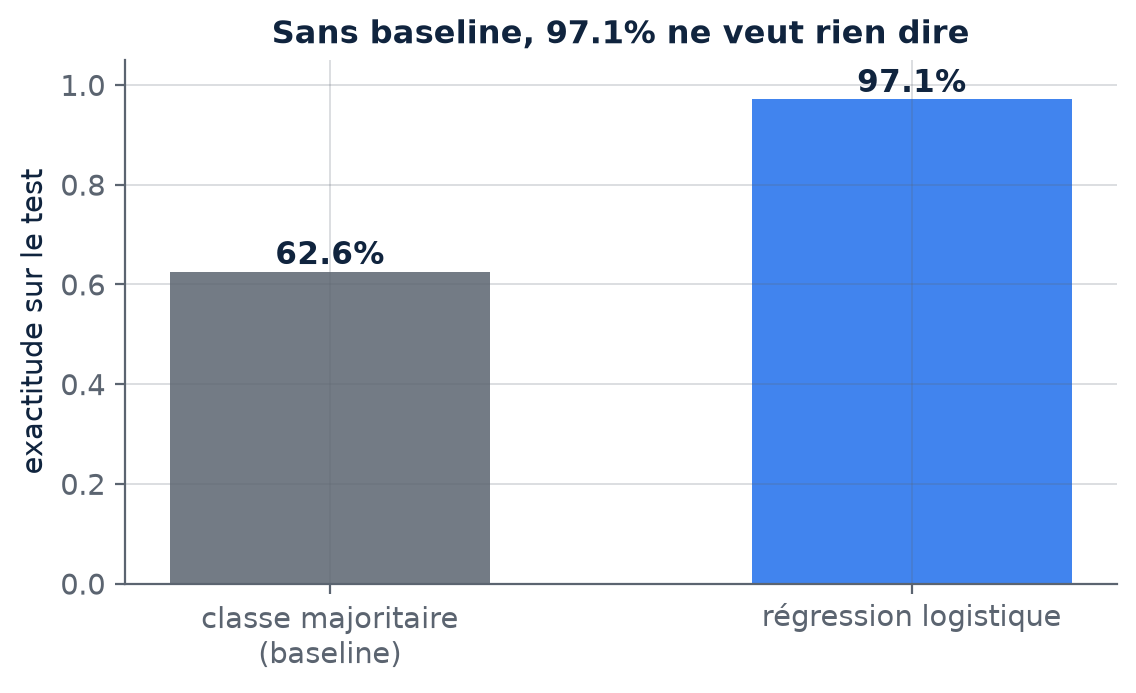
\includegraphics[width=0.82\textwidth]{g08_baseline.png}
\end{column}
\begin{column}{0.50\textwidth}
\begin{itemize}
  \item Classe majoritaire seule : \textbf{62,6 \%}.
  \item Régression logistique : \textbf{97,1 \%}.
  \item Gain réel : \textbf{+34,5 points}.
\end{itemize}
\begin{wbox}[Sans baseline]
« 97 \% » impressionne. « +34,5 points par rapport à la classe
majoritaire » informe.
\end{wbox}
\end{column}
\end{columns}
\vspace{1mm}
{\footnotesize\color{byGrey}Trois baselines à essayer : classe majoritaire
(ou moyenne), dernière valeur pour une série, modèle linéaire simple.}
\end{frame}

\begin{frame}{Quiz 2 --- évaluation}
\begin{qbox}[Question 1]
Vous standardisez les variables sur tout le jeu, puis vous découpez. Que
fabriquez-vous ?
\begin{itemize}
  \item[(a)] une fuite de données \quad (b) un meilleur modèle \quad
  (c) rien de particulier
\end{itemize}
\end{qbox}
\begin{qbox}[Question 2]
Le jeu de test sert à :
\begin{itemize}
  \item[(a)] choisir les hyperparamètres \quad (b) estimer la performance
  finale, une seule fois \quad (c) entraîner le modèle
\end{itemize}
\end{qbox}
\begin{qbox}[Question 3]
Un modèle atteint 99 \% sur des données bruitées. La réaction correcte est :
\begin{itemize}
  \item[(a)] publier le résultat \quad (b) chercher la fuite \quad
  (c) ajouter des couches
\end{itemize}
\end{qbox}
\begin{solbox}[Réponses]
\textbf{1.} (a). \quad \textbf{2.} (b). \quad \textbf{3.} (b) : un score
au-delà du bruit irréductible signale une erreur de protocole.
\end{solbox}
\end{frame}
